% ---------------------------------------------------------------------
% Drop-in for Sec. VIII: verification of the error analysis on the
% campaign.  Place after the offset results.
%
% The figure is docs/fig_sec8_error.png, regenerated by
%     python analysis/mcrit_repeatability.py DataSet/exp
%     python analysis/fit_quality_bound.py   DataSet/exp
%     python analysis/sec8_figure.py docs/fig_sec8_error.png
% (the first two write the caches the third reads).
%
% The section deliberately keeps two kinds of number apart and says so:
% (108) is a GUARANTEE on one term, the repeatability is a MEASUREMENT of
% the whole.  Merging them into a single accuracy figure would misstate
% both.  Renumber equations to match the host document.
% ---------------------------------------------------------------------

\documentclass[10pt]{article}
\usepackage[a4paper,margin=22mm]{geometry}
\usepackage{amsmath,amssymb,booktabs,graphicx}
\setlength{\parskip}{0.35em}\setlength{\parindent}{0pt}
\newcommand{\Mdot}{\dot M}
\newcommand{\rbar}{\bar\rho}
\title{\vspace{-16mm}\textbf{Sec.~VIII-x: the error analysis, verified on
the campaign}\vspace{-3mm}}
\date{\small drop-in; figure \texttt{fig\_sec8\_error.png}}
\begin{document}\maketitle

\begin{figure}[t]
\centering
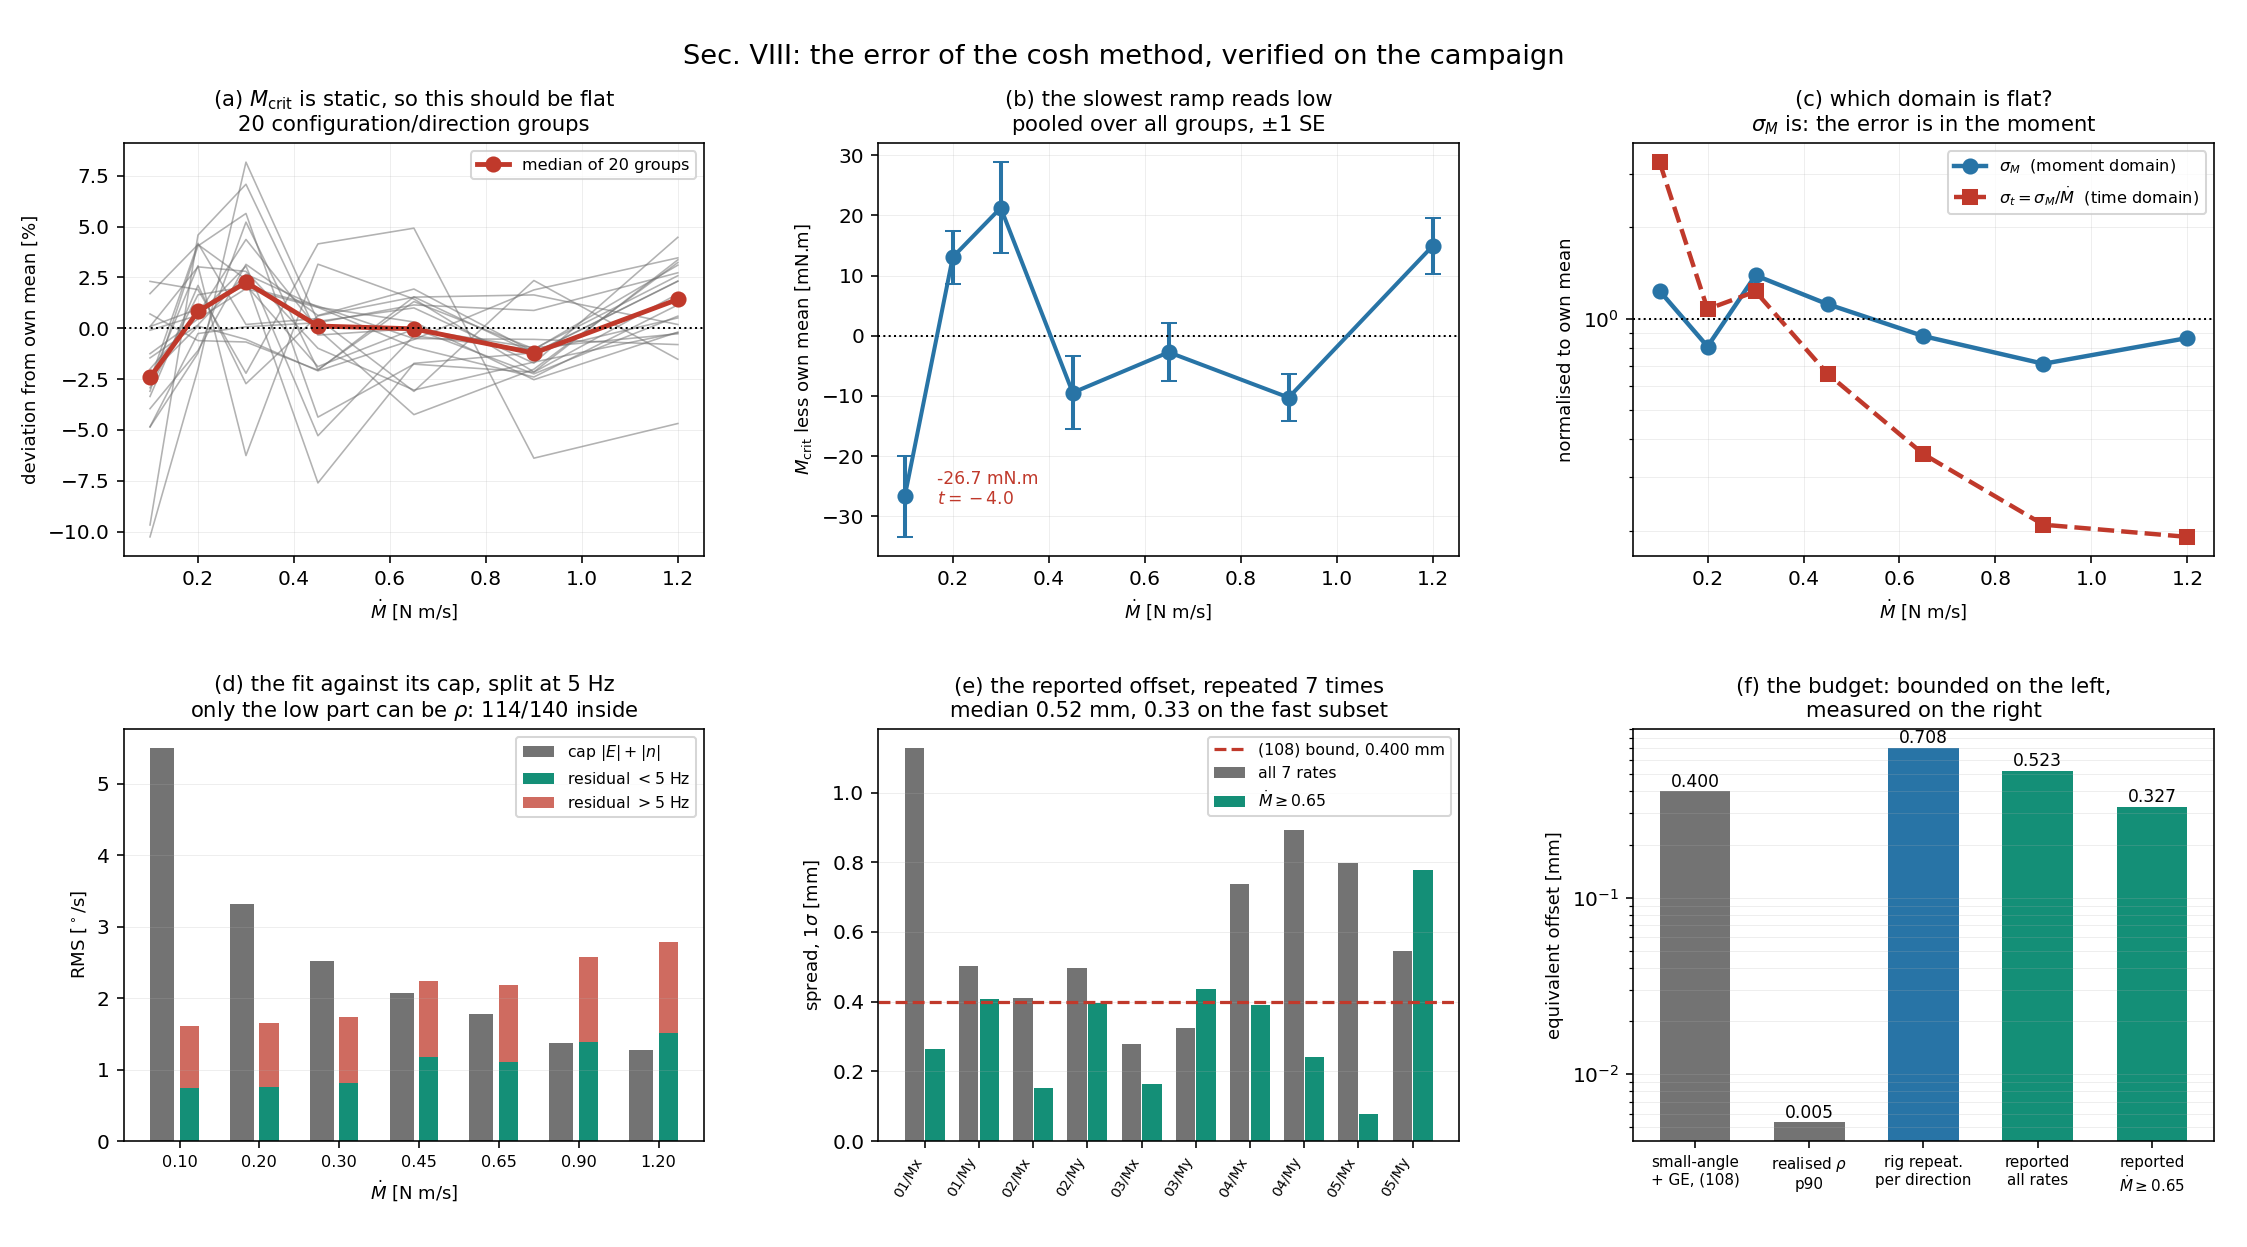
\includegraphics[width=\linewidth]{fig_sec8_error.png}
\caption{The error of the identification, measured on the $140$-run
campaign. \emph{(a)} the identified critical moment against the ramp
rate for all twenty configuration/direction groups, each scaled by its
own mean; $M_{\rm crit}$ is a static property of the rig, so the ideal
is a flat line and every departure is error, with no model in the
comparison. \emph{(b)} the same pooled by rate: only the slowest ramp
departs significantly. \emph{(c)} the domain test --- $\sigma_M$ is flat
and $\sigma_t = \sigma_M/\Mdot$ is not, so the dominant error is in the
moment rather than in the located onset. \emph{(d)} the fit residual
against its a priori cap, split at $5$~Hz; only the low-frequency part
can be the modelling remainder. \emph{(e)} the reported half-sum,
repeated at seven rates per configuration, against the bound of (108).
\emph{(f)} the budget, bounded terms on the left and measured ones on
the right.}
\label{fig:sec8-error}
\end{figure}

\subsection{What is guaranteed, and what is measured}

Two different kinds of statement are made about the accuracy of the
identification and they must not be merged. Equation (108) is a
\emph{guarantee}: given a scale, a CAD inertia and the excitation
protocol, the terms the model neglects cannot displace the identified
threshold by more than $\rbar$, which is $12.04$~mN\,m for roll and
$9.95$ for pitch, or $0.400$ and $0.322$~mm of equivalent offset. It
says nothing about sensor noise, rig repeatability or anything else it
did not model. The repeatability reported below is a \emph{measurement}
of the whole error, with no model in it at all. Quoting either as if it
were the other would misstate both.

\subsection{The bound, checked forwards}

The guarantee is verified as described in
Sec.~\ref{sec:bound-check}: each perturbation is evaluated along the
measured trajectory, propagated through the deviation dynamics and
correlated against the weight of (107). All $140$ runs fall inside,
with a median displacement of $0.049$~mN\,m, $0.161$ at p90 and $0.927$
at worst against the $12.04$ allowed.

That margin is not an accident and it has a closed form. Writing
$x = C_2\tau_{\rm end}$, the gravity remainder behaves as
$\rho_\varphi\propto\varphi^2\sim e^{2C_2 s}$ near the window end, so
$e_\omega\sim e^{2x}$ while $\rbar\sim e^{2x}/x$ and therefore the
envelope of (93) grows as $E\sim e^{3x}/x$:
\begin{equation}
  \frac{|e_\omega|}{E}\;\sim\;x\,e^{-x} .
  \tag{VIII.1}
\end{equation}
Both grow with the window; the bound grows by one whole factor of
$e^{x}$ more, because the Chebyshev step of (93) puts the window average
of $\rho$ underneath a kernel that is largest exactly where $\rho$ is
smallest. Equivalently, keeping the covariance that Chebyshev discards
turns the inequality into an identity,
\begin{equation}
  \frac{|e_\omega|}{E}
   = 1 + \operatorname{corr}(\rho,h_\omega)\,
         \mathrm{CV}_\rho\,\mathrm{CV}_{h} ,
  \tag{VIII.2}
\end{equation}
and lengthening the window makes both coefficients of variation grow
faster than the correlation weakens. Measured, the realised deviation is
$3.2\%$ of the bound at $\Mdot = 0.10$ and $20.8\%$ at $1.20$; the
reduction factors evaluated at their suprema account for a further
factor of $1.5$ to $2.1$, roughly constant across the rates.

This says how informative the guarantee is and nothing else, and the
distinction is worth making explicitly because the two are easily
conflated. A larger occupancy means the bound is closer to the truth,
not that the truth is larger or smaller. On the $\rho$ channel the fast
ramp is in fact slightly \emph{worse}: the deviation is less aligned
with the onset direction there ($31.4^\circ$ against $23.0^\circ$, so
$82\%$ of it is absorbable rather than $89\%$), but
$\Delta M_{\rm crit} = \Mdot\,\delta$ and $\delta$ falls only
$2.3\times$ across the rate range while $\Mdot$ rises twelvefold, so the
channel contributes $0.35$~mN\,m at $\Mdot = 0.10$ and $1.82$ at
$1.20$. The recommendation on excitation rate is made separately below,
on measured grounds, and does not rest on this paragraph.

\subsection{The fit against its cap}

Because the nominal response is itself an admissible member of the
fitted family, the minimiser cannot do worse than it does, and with the
sensor noise added by the triangle inequality
\begin{equation}
  \|\hat r\| = \min_g\|y-g\| \le \|y-f\| \le \|e_\omega\| + \|n\|
             \le \|E\| + \|n\| .
  \tag{VIII.3}
\end{equation}
The comparison needs the residual split first. $e_\omega$ is a Duhamel
integral of a smooth $\rho$ and carries essentially nothing above a few
times $1/\tau_{\rm end}$, so residual content faster than that cannot be
the small-angle or ground-effect remainder whatever else it is; charging
the model for it is not a test of the model. Splitting at $5$~Hz (the
windows are $53$ samples at $100$~Hz, too short for an IIR filter), the
low-frequency residual lies inside the cap for $114$ of $140$ runs, the
$26$ exceptions all at the two fastest rates and by no more than a
factor $1.16$. Including the high-frequency content the figure is
$88/140$.

The split also identifies what the rest is. Above $5$~Hz the residual
carries $1.02^\circ$/s while the pre-onset record carries $0.14$, a
factor of seven: before the onset the vehicle is supported by every
landing gear and after it pivots on one edge with far less damping, so
the pre-onset floor understates the in-window disturbance and must not
be used as $\|n\|$.

\subsection{Repeatability, with no model in it}

The campaign supplies a model-free accuracy measurement, because
$M_{\rm crit}$ is a \emph{static} property of the rig --- the moment at
which the vehicle is on the verge of tipping over a landing-gear edge
--- and cannot depend on how fast the moment was ramped to reach it.
Identifying it at seven rates per configuration and per direction
therefore repeats a measurement whose true value is known to be
constant, and Fig.~\ref{fig:sec8-error}(a) is that test.

\begin{center}\small
\begin{tabular}{@{}lrr@{}}
\toprule
 & per direction & reported half-sum \\
\midrule
scatter $\sigma_M$ & $21.3$~mN\,m & --- \\
as equivalent offset & $0.71$~mm & --- \\
$1\sigma$ across the rates & --- & $0.28$ to $1.13$~mm \\
median & --- & $0.522$~mm \\
median, $\Mdot\ge0.65$ & --- & $0.327$~mm \\
\bottomrule
\end{tabular}
\end{center}

The two columns are consistent with each other without adjustment: two
directions with independent moment-domain errors give a half-sum spread
of $\sigma_M/\sqrt2 = 0.50$~mm, and the measured median is $0.522$.

\paragraph{Which domain.} A mislocated onset is an error in \emph{time},
so it would show a flat $\sigma_t$ and a $\sigma_M$ rising with $\Mdot$;
a vehicle that does not tip at exactly the same moment twice is an error
in \emph{moment}, so $\sigma_M$ is flat and $\sigma_t$ falls as
$1/\Mdot$. Measured, $\sigma_M$ runs $13.7$ to $33.5$~mN\,m with a
coefficient of variation of $34\%$ while $\sigma_t$ runs $11.4$ to
$225$~ms at $97\%$: the error is in the moment.

The alternative can be excluded quantitatively rather than by
inspection. If the scatter were a within-run disturbance seen through
the onset, then for a disturbance of fixed amplitude
$\sigma(\Delta M_{\rm crit}) \propto \sqrt{C_2/B(x)}$, so the short
window --- the fast ramp --- would scatter \emph{more}, by a factor
$5.72$ across the rate range. It scatters $0.70$, an eightfold
disagreement in the opposite direction. The scatter is a run-to-run
change in where the vehicle actually tips: landing-gear settling, floor
friction and repositioning between runs.

\paragraph{The slowest ramp.} One condition departs systematically.
Pooling the identified $M_{\rm crit}$ less each configuration's own mean,
$\Mdot = 0.10$~N\,m/s reads $-26.70$~mN\,m against $+4.45$ for the rest
(Welch $t = -4.34$, $p = 0.0002$), with $75\%$ of those runs below their
own mean. As an onset error that is $267$~ms, matching the $225$~ms of
$\sigma_t$ measured there, and its sign says the onset is found
\emph{early} --- what a slow rise emerging from noise does to a residual
minimiser. It is not $\rho$, which contributes $0.3$ to $1.8$~mN\,m on
these channels, twenty times too small and with the opposite rate trend.
Restricting the protocol to $\Mdot\ge0.65$~N\,m/s removes it and takes
the reported spread from $0.522$ to $0.327$~mm.

\subsection{What the two-sided difference removes}

The offset is read from the half-sum $M_{\rm off} = (M_+ + M_-)/2$, and
the two runs tip over different edges with restoring arms
$A_\pm = l_p\mp a$. In mirrored coordinates both obey the same equation,
so in signed $\varphi$ the arm term of the deviation forcing carries
$\operatorname{sign}(\Mdot)$ while the $Wz\sin\varphi$ term does not: the
arm term is antisymmetric and cancels. Simulating the full nonlinear
tip-over with a $2$~mm offset and fitting with the deployed estimator,
$98.70\%$ of the per-direction bias cancels at every rate, leaving about
$1~\mu$m. The ground-effect channel cancels as well: $\beta_M$ flips
sign with the pivot edge --- it is proportional to
$\sum_i (l_{y,i}+l_p)^2 b^\dagger_{i,\varphi}$, and the allocation basis
reverses --- so the bilinear term of (79) is odd and contributes
$0.6$ to $0.9~\mu$m instead of the $46$ to $78$ it would if it were
even. The per-configuration calibration cancels too, being common to
both directions by construction: $\pm10\%$ of amplitude error and
$\pm5\%$ of exponent error are rejected to $99.77$--$99.98\%$ and move
the offset by $0.000$~mm.

What does not cancel is the weight, because (34) reads the
\emph{difference} of the two critical moments, where the same bias adds.
Per $1\%$ of calibration error that is $0.027\%$ of $W$ from the
amplitude channel and $0.077\%$ from the exponent, the exponent being
the more damaging by about three; the closed forms are
$A(x)/B(x)$ and $D(x)/B(x)$ times $\Mdot/C_2$.

\subsection{Choosing the excitation rate}

The protocol's seven rates permit the choice to be made on measurement
rather than argument. Taking each configuration's half-sum at a given
rate against its own mean over all rates isolates the error contributed
by that rate:

\begin{center}\small
\begin{tabular}{@{}rrrrr@{}}
\toprule
$\Mdot$ & post-onset & window & RMS error & p90 \\
N\,m/s & samples & s & mm & mm \\
\midrule
$0.10$ & $74$ & $0.740$ & $0.810$ & $1.035$ \\
$0.20$ & $64$ & $0.635$ & $0.569$ & $0.975$ \\
$0.30$ & $58$ & $0.575$ & $0.708$ & $0.994$ \\
$0.45$ & $54$ & $0.545$ & $0.707$ & $1.374$ \\
$0.65$ & $48$ & $0.480$ & $0.528$ & $0.924$ \\
$0.90$ & $44$ & $0.445$ & $0.443$ & $0.696$ \\
$1.20$ & $41$ & $0.410$ & $\mathbf{0.422}$ & $\mathbf{0.637}$ \\
\bottomrule
\end{tabular}
\end{center}

There is no interior optimum: the error falls to the fastest rate
tested. That is worth checking against the obvious objection, which is
that a faster ramp shortens the window and leaves fewer samples to fit.
It does --- $74$ down to $41$ --- but the onset is located by
$\|\chi\|^2 = C_1^2C_2B(x)$ with $C_1 = \Mdot/W\!z_{CoM}$, so the
amplitude rises twelvefold while the sample count falls only $1.8\times$,
and the product improves: $\|\chi\|$ grows $1.35\times$ and the onset
uncertainty $\sigma_\delta$ falls by $26\%$. Forty-one samples remain
ample for a two-parameter fit.

Two effects would eventually create an interior optimum and neither has
taken over by $1.20$~N\,m/s. The onset is quantised to the sample grid,
contributing $T_s\Mdot/\sqrt{12}$ per direction, or $0.081$~mm to the
half-sum at the fastest rate against the $0.422$ measured --- under
$4\%$ of the variance, and removable outright by refining the onset
below the grid. And the pseudo-inverse allocation saturates at
$M_{x,\max} = 2.371$ and $M_{y,\max} = 2.737$~N\,m (Figs.~13--14),
which caps the usable rate from above. Within the range tested the
recommendation is simply the top of it, and restricting to
$\Mdot\ge0.65$~N\,m/s takes the reported spread from $0.522$ to
$0.327$~mm.

\subsection{Summary}

\begin{center}\small
\begin{tabular}{@{}llr@{}}
\toprule
term & how known & equivalent offset \\
\midrule
small-angle $+$ GE remainder & bounded a priori, (108) & $\le 0.400$~mm \\
\quad realised, p90 & forward check, $140/140$ & $0.005$~mm \\
onset location & not resolved; below the next line & --- \\
rig repeatability, per direction & measured & $0.71$~mm \\
\midrule
\textbf{reported offset, all rates} & measured, $7\times$ per config
  & $\mathbf{0.522}$~mm \\
\textbf{reported offset, $\Mdot\ge0.65$} & measured & $\mathbf{0.327}$~mm \\
\bottomrule
\end{tabular}
\end{center}

The modelling approximations are therefore a bounded minority of an
error the rig dominates: whatever limits this method, it is not the
neglected $\sin\varphi$. That is worth stating plainly because it also
justifies the change of onset model. The quadratic growth law used
previously carried a \emph{systematic} error of $12$ to $31\%$ of the
window in the located onset --- $22$ to $58$~mN\,m over the observed
$x$ range, comparable to or larger than the entire error measured here,
and a bias rather than a scatter, so averaging does not reduce it.
Retaining $Wz_{CoM}\varphi$, which is exactly what turns the quadratic
into the hyperbolic cosine with $C_2^2 = Wz_{CoM}/J_P$, moves the
algorithm's contribution from dominant to negligible.

\end{document}
